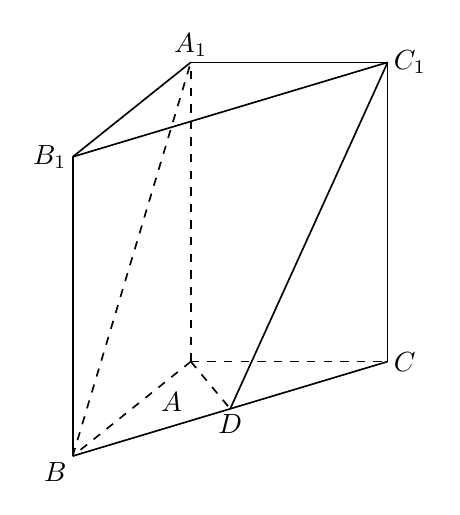
\begin{tikzpicture}[x=1cm,y=1cm,font=\normalsize,
  edge/.style={draw=black,solid,line width=.6pt},
  hide/.style={draw=black,dashed,line width=.6pt}]
% Upright triangular prism A1B1C1-ABC, D midpoint of BC
\coordinate (A) at (0.0,0.0);
\coordinate (B) at (-1.5,-1.2);
\coordinate (C) at (2.5000000000,0.0000000000);
\coordinate (D) at (0.5000000000,-0.6000000000);
\coordinate (A1) at (0.0000000000,3.8000000000);
\coordinate (B1) at (-1.5000000000,2.6000000000);
\coordinate (C1) at (2.5000000000,3.8000000000);
% solid verticals and top
\draw[edge] (B)--(B1);
\draw[edge] (C)--(C1);
\draw[edge] (B)--(D);
\draw[edge] (D)--(C);
\draw[edge] (A1)--(C1);
\draw[edge] (B1)--(C1);
\draw[edge] (A1)--(B1);
\draw[edge] (C1)--(D);
% hidden prism edges and auxiliary lines
\draw[hide] (A)--(A1);
\draw[hide] (A)--(B);
\draw[hide] (A)--(C);
\draw[hide] (A)--(D);
\draw[hide] (B)--(A1);

\node[below left,inner sep=2pt,xshift=-1pt,yshift=-9pt] at (A) {$A$};
\node[below left,inner sep=2pt] at (B) {$B$};
\node[right,inner sep=2pt] at (C) {$C$};
\node[below,inner sep=2pt] at (D) {$D$};
\node[above,inner sep=2pt] at (A1) {$A_{1}$};
\node[left,inner sep=2pt] at (B1) {$B_{1}$};
\node[right,inner sep=2pt] at (C1) {$C_{1}$};
\end{tikzpicture}
